\scanpage{60}
On voit alors que
\[
x\prec y\text{ et }y\prec z\quad\Longrightarrow\quad x\prec z
\]
car soient $u,v\in\unsure{\Sigma_{<}(1)|\Sigma^{<}(1)}$ tels que
\[
p_1u=x,\quad\underbrace{\uline{b}u=y,\quad p_1v=y},\quad\uline{b}v=z
\]
on a donc
\[
\uline{b}u=p_1v
\]
donc par le carré cartésien de (38), \deleted{$\unsure{\exists u}$}
\[
\unsure{\exists!|\exists\mid}\ d\in\Sigma^{<}(2),\quad\text{avec}\quad\uline{b'}(d)=v,\quad p_2(d)=u
\]
soit
\[
w=\uline{s'}(d)\in\Sigma^{<}(1)
\]
on a
\[
\begin{aligned}
p_1(w)&=p_1(\uline{s'}(d))\overset{(38)}{=}p_1p_2(d)=p_1(u)=x\\
\uline{b}(w)&=\uline{b}(\uline{s'}(d))=\uline{b}(\uline{b'}(d))=\uline{b}(v)=z
\end{aligned}
\]
donc
\figure{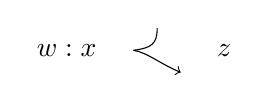
\begin{tikzpicture}[baseline=(x.base)]
\node (x) at (0,0) {$w:x$};
\node at (2,0) {$z$};
\draw (1.15,.28) .. controls (1.15,.08) and (1.08,.03) .. (.85,0);
\draw[->] (.85,0) .. controls (1.03,-.03) and (1.2,-.18) .. (1.45,-.28);
\end{tikzpicture}}.
De plus, on a
\[
x\not\prec x\qquad\left(\text{car }\operatorname{Im}(\Sigma_1\overset{(p_1;\uline{b})}{\unsure{-|\longrightarrow}}\Sigma\times\Sigma)\cap\text{diag}=\varnothing\right)
\]
donc la relation $x\prec y$ est la relation
d'inégalité stricte associée à une relation
d'ordre sur $\Sigma$. On récupère $\Sigma^{<}(1)$ comme
le graphe de la relation d'ordre stricte,
$\Sigma^{<}(2)$ comme les drapeaux $x\prec y\prec z$ de
longueur $2$ dans $\Sigma$, et les applications
\mspage{59}
